\documentclass[a4paper,12pt]{article}

\usepackage{url, hyperref, graphicx}

\begin{document}

\title{Project 2}
\author{Chip Bell}
\date{April 24, 2015}
\maketitle

\section{Problem Description}
The Washington Metropolitan Area Transit Authority's Metrorail system in many respects is a driving factor in the
expansion of the city. With Washington's fixed size, reliable and cost-efficient transportation for metro area
residents is crucial for maintaining the city's economy. However, this is a difficult task in that there are many
variables involved, such as human error, mechanical failure, and even acts of nature.

Therefore for this project, I will be simulating the metrorail system using data collected from the WMATA API
\cite{wmataapi}, which provides realtime estimates of train arrival. Furthermore, I will simulate the impact that track
closures have on train throughput.

\section{Previous Work}
Many large cities have rapid transit systems, so considerable research time has been invested on building reliable
subways. Commercial software such as OpenTrack \cite{opentrack} have been developed, and even video games such as Train
Simulator \cite{trainsimulator} and Open Rails \cite{openrails}. Algorithms for handling single, double and triple tracks exist,
such as a basic
algorithm for sharing tracks between trains presented by Fiorini and Botter \cite{fioroni}. Dessouky and Leachman
\cite{dessouky_leachman_95} provide an event-driven algorithm for single and double track rail networks, incorporating
acceleration. Lu et al \cite{quan_lu} expand the model to triple tracks while enhancing the acceleration model to
handle multiple track speed limits.

\section{Basic Architecture}
The nature of trains lends itself to a model that incorporates resource sharing. For instance, only a single train can
occupy a particular section of track at a given moment. Furthermore, if two trains are sharing a track, they cannot
be going in different directions unless they have already past each other, lest they collide. This issue is addressed
by Fioroni \cite{fioroni}.

A common occurrence in the metro system is that between two stations a particular section of track is under
maintenance, forcing trains going both directions to share a track. These basic issues result in a couple of clear
concepts that we'll incorporate in our model.

The first is a train. A \texttt{Train} encapsulates all of the information relevant to our application: which line it is
(Orange, Blue, or Silver), it's direction, and it's location within the system. Measuring the throughput of trains
in the system will be our primary statistic when running the simulation.

The other important entity to be concerned with is the track itself. In the simulation, this is modeled using a
\texttt{TrackSegment} class. A \texttt{TrackSegment} is simply a queue with the ability to be process \texttt{Train}s
one at time.

From a queueing standpoint, a \texttt{TrackSegment} is a limited
resource that only a single train can use at a single point. If a piece of track is occupied by a train, all other
trains must wait before they may proceed through the track (in an assumed FIFO order). It is for this reason that
most train systems do prefer to have a second track to prevent blocking for trains going in opposite directions.
So, in our case we can treat a section of track as a queue that can only process a single train at a time. Between
stations, there are generally two sections of track. However, track maintenance would cause a track to close, forcing
opposing tracks to share.

Because of this, we can represent the entire metro as queuing network with sections between stations as the queue. In
our case, we will only be modeling the section of track between Rosslyn and Stadium-Armory where the Orange, Blue, and
Silver share a track (See \ref{fig:metromap}) which results in a simpler network with the nodes falling in a single
line. Since there are no track crossovers within the DC metro, we can consider these three lines
to be isolated from other lines, so we lose no accuracy by excluding the other lines from the simulation. However, we
do need to keep in mind that for two tracks, each track is devoted to a specific direction. Only in the case of a single
track is when a track will handle both directions.

I've also chosen to conceptually model pairs of tracks between stations as a \texttt{StationConnection} class. Perhaps
unsurprisingly, this is the largest and most important class in the simulation, since it manage two
\texttt{TrackSegment}s, along with the disabling/enabling of a track segment. When a track is disabled, the
\texttt{StationConnection} must begin routing trains through a single track, rather than reserving tracks for
only particular directions. This logic is important to the accuracy and realism of the simulation, since it's one of
fundamental principles behind a train track. 

Because this will be a discrete-event simulation, we will need to be mindful of the events that travel through our
application. A first example that comes to mind is the \texttt{train:arrive} event, which will be received by the
Rosslyn and Stadium-Armory stations when a train first arrives in the system. This event will need to contain the train
instance, along with the direction its heading. This way, we can
track the train as it moves through the system to calculate metrics about the system's performance.

When a train first arrives at a station, it is queued up to await a free track. If the track designated for that
direction is already available, the train simply moves on to the track and occupies it until it reaches the next
station where it exits and then queues up at the next station.

When a train is dequeued and allowed to enter a track, a \texttt{train:enter} event is thrown. When this event occurs,
the station connection marks the track as occupied so that later arriving trains do not attempt to enter the track. The
connection also schedules a new event: \texttt{train:exit}

\texttt{train:exit} is triggered when a train exits a connection, which informs a connection to free up the track and
push the next train through, if there is one. As mentioned before, this event is actually scheduled when a train enters
a track between stations. Each connection has knowledge of the time between it's associated stations, and uses that
time to schedule the \texttt{train:exit} in relation to \texttt{train:enter} for a particular train. Lastly, when a
train exits a particular connection, a \texttt{train:arrive} event is scheduled immediately for the next connection in
the metro system.

\begin{figure}
\begin{center}
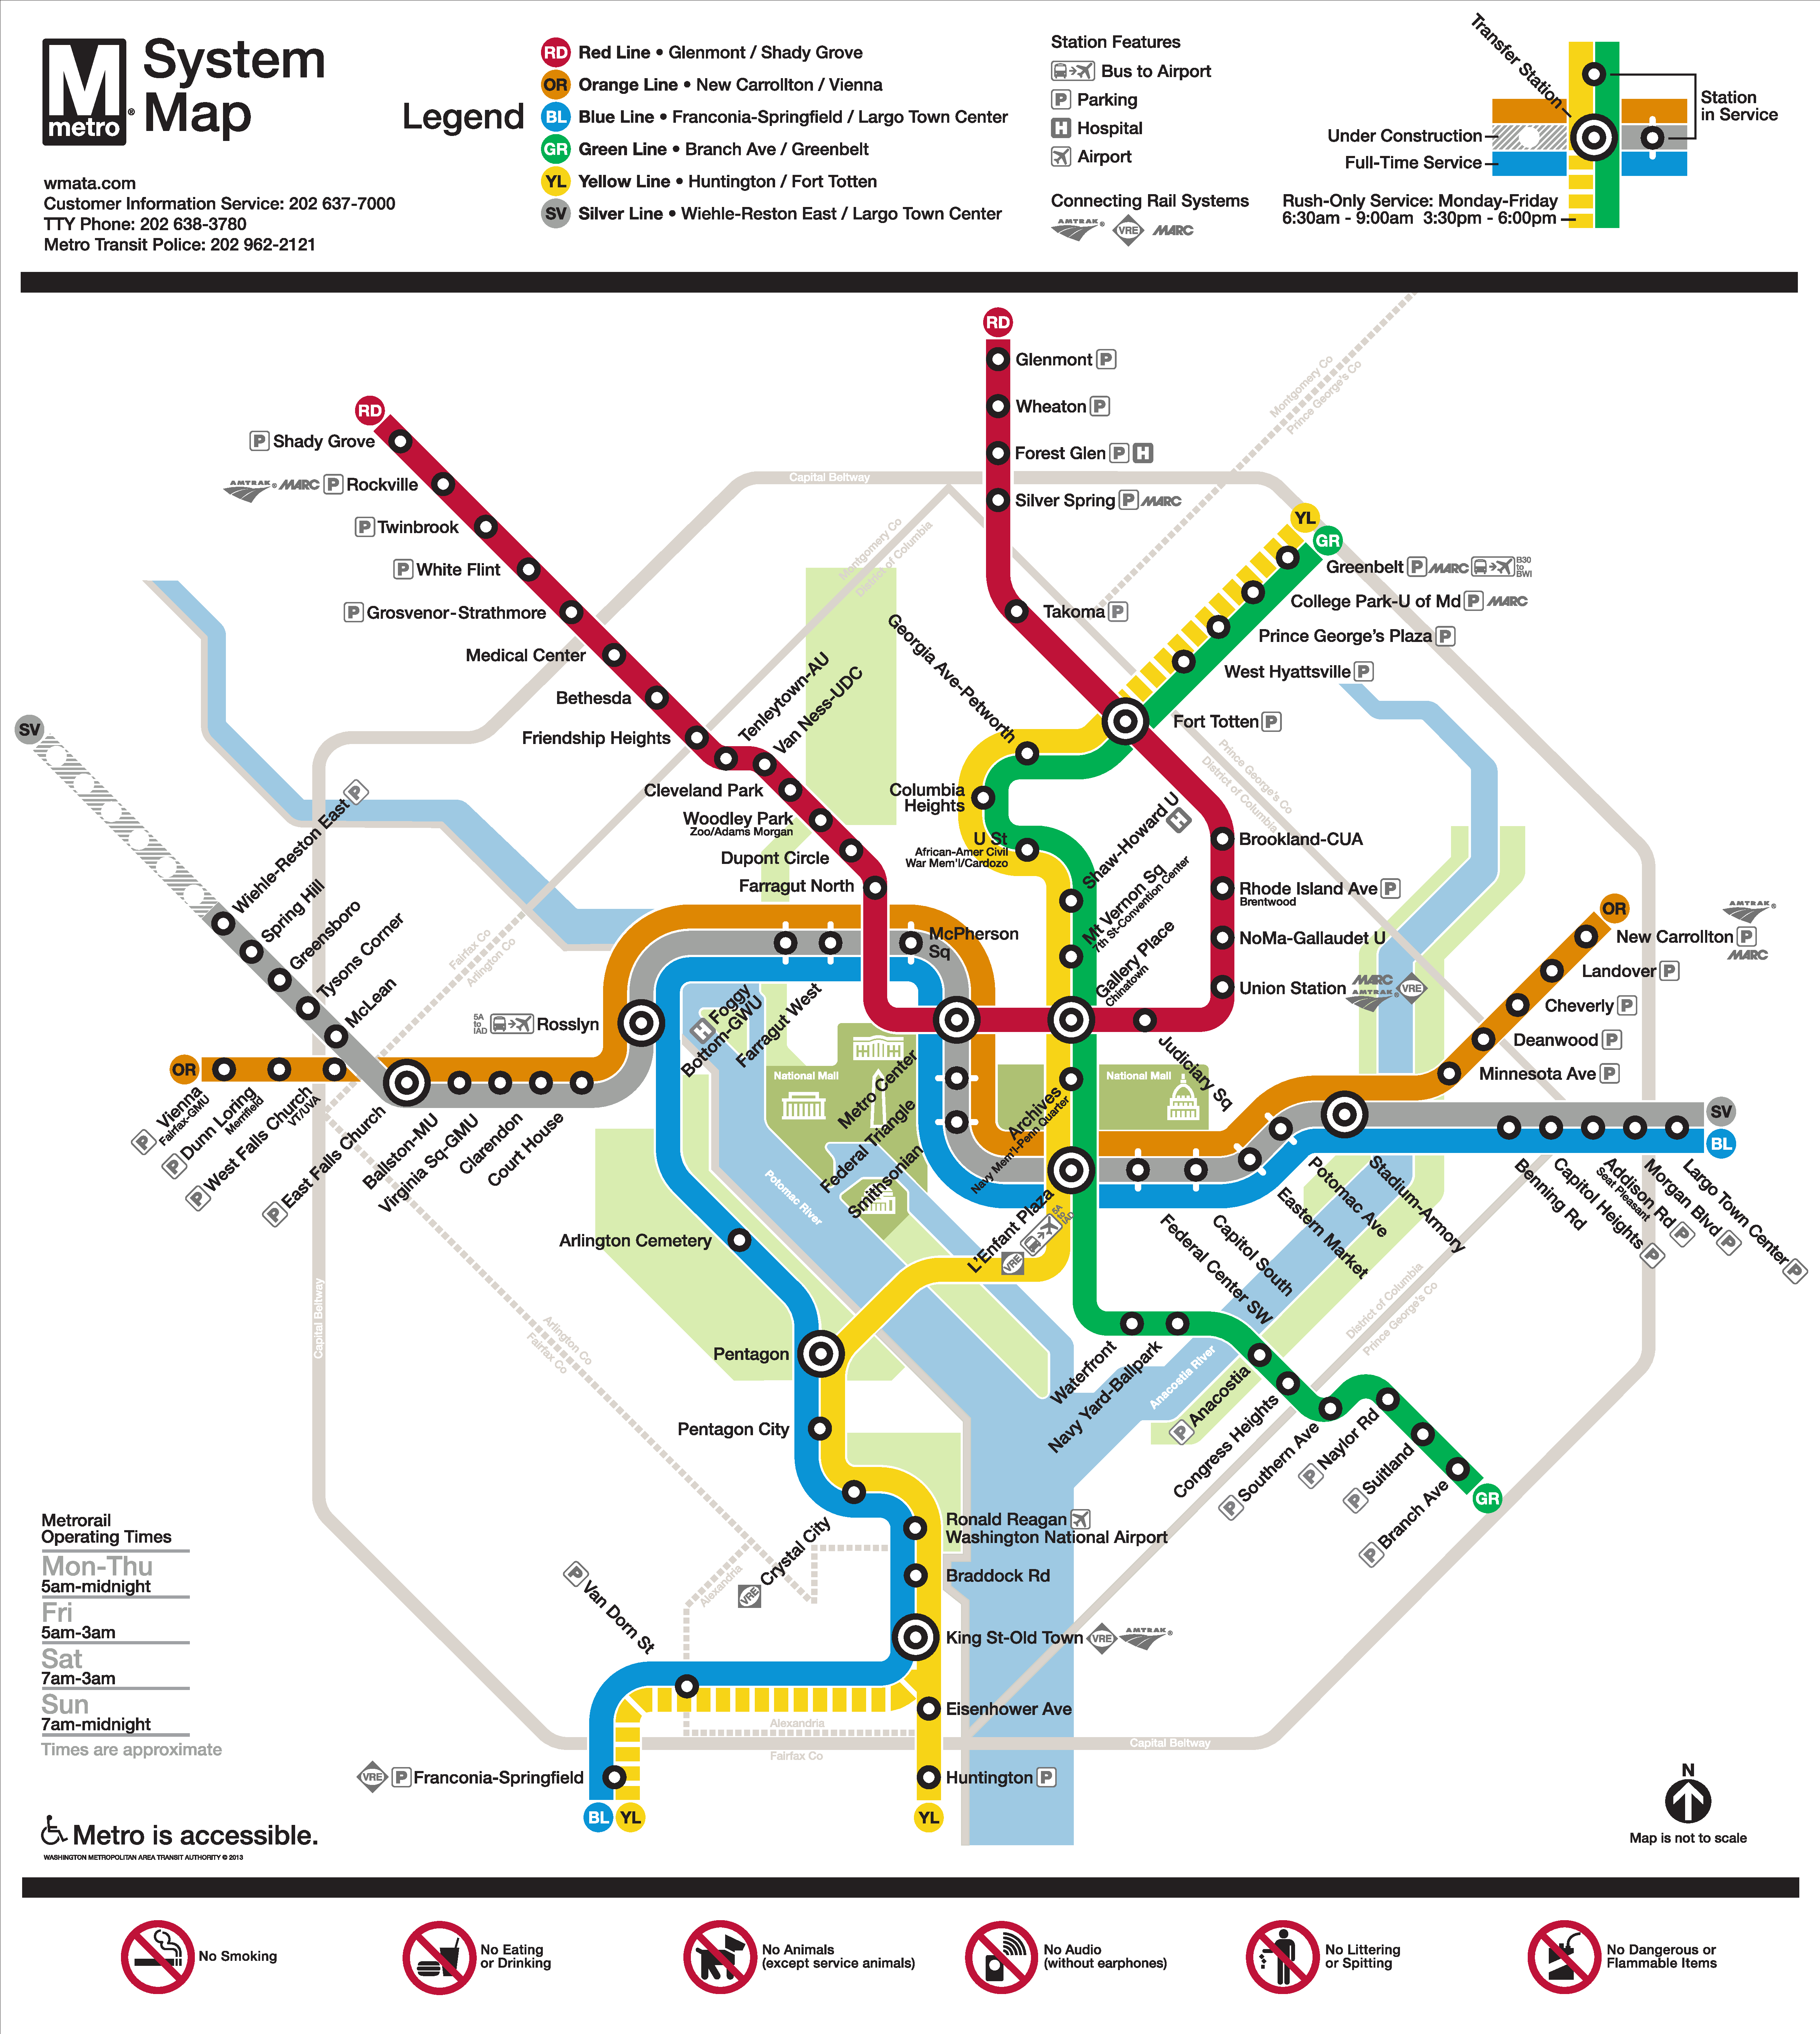
\includegraphics[width=5in]{../images/metro_map.pdf}
\caption{\small \sl WMATA Metrorail Map \label{fig:metromap} \cite{fioroni}}
\end{center}
\end{figure}

\section{Data Collection}

\subsection{Query Design}
Viewing this as a queueing problem, there are some ``missing pieces'' that our model did not incorporate, namely the
arrival rate of trains and the service time for a single train. Instead of attempting to calculate these based on 
numerical models of motion, we can instead use the WMATA API \cite{wmataapi} to claculate an empirical value.

The API provides data by station with an estimate at each station of the wait time until the next train. For instance,
the API for a station on the blue line might list a train to Franconia-Springfield (westbound) in 1 minute. If there
also happens to be an Orange that passes through that station, you may also see an estimate for the next Orange (if it
is close enough).

Given this information, we can calculate how often a train runs simply by marking the timestamp of the API call and
offset by the estimated time until arrival provided by the API. For instance, if we query a station at 12:00 PM, and
the API estimates a train arriving in 3 minutes, we can roughly estimate that the train will arrive at 12:03.
Performing this operation over time gives us a list of train arrival time by station from which we can calculate
interarrival time via a running diff. Furthermore, we can query by train line as well to verify that trains run
according to the schedule that WMATA provides on its website \cite{metroschedule}.

To calculate service times for a particular section of track, we need an estimate of the time it takes for a train to
travel between two stations. This is clearly station dependent, since some stations are closer than others. However,
all but one of our stations are within the District of Columbia, so we expect the travel times to be small.

We can still calculate an estimated travel time between two stations through the API as well. Given two neighboring stations $A$ and $B$, if
we query $A$ for an upcoming trains of color $c$ in the direction of $B$, we will get some estimate for the arrival. We
can query $B$ for the same color train in the same direction to obtain a estimate of the arrival time at $B$.
Subtracting these two numbers provides an estimate of the travel time between stations. This makes an assumption that
there is no train of the same color in the middle that may skew the estimate. However, we can minimize the chance of
this happening if we restrict our queries on $A$ to trains that are only a minute away. Given that the stations are so
close, we minimize the likelihood that there is a ``middle train'' that causes inaccurate estimates.

\subsection{Query Results}
A script was built to call the WMATA API for train estimates, and was setup as a cron job on a server and scheduled to
run every minute for a week. The script
essentially downloaded the estimates of train arrivals for every station into a single timestamped JSON file (see the
JSON format \cite{json}. Cron \cite{crontab} was configured to run the script every minute for an entire week,
resulting in a directory full of timestamped JSON files. These were then imported into a MongoDB \cite{mongodb} database 
to allow easier queries.

Train interarrivals were measured by line and direction. (\ref{fig:eastboundblueinterarrivals}) demonstrates that the
data oftentimes appears to follow some ``standard'' distribution. However, other cases such as
(\ref{fig:westboundsilverinterarrivals}) show that this is not necessarily true. Graphs for the remaining directions
and line colors were omitted for brevity, but are included in
the submission. Due to time constraints, we'll use an empirical distribution rather than trying to fit any particular
distribution.

\begin{figure}
\begin{center}
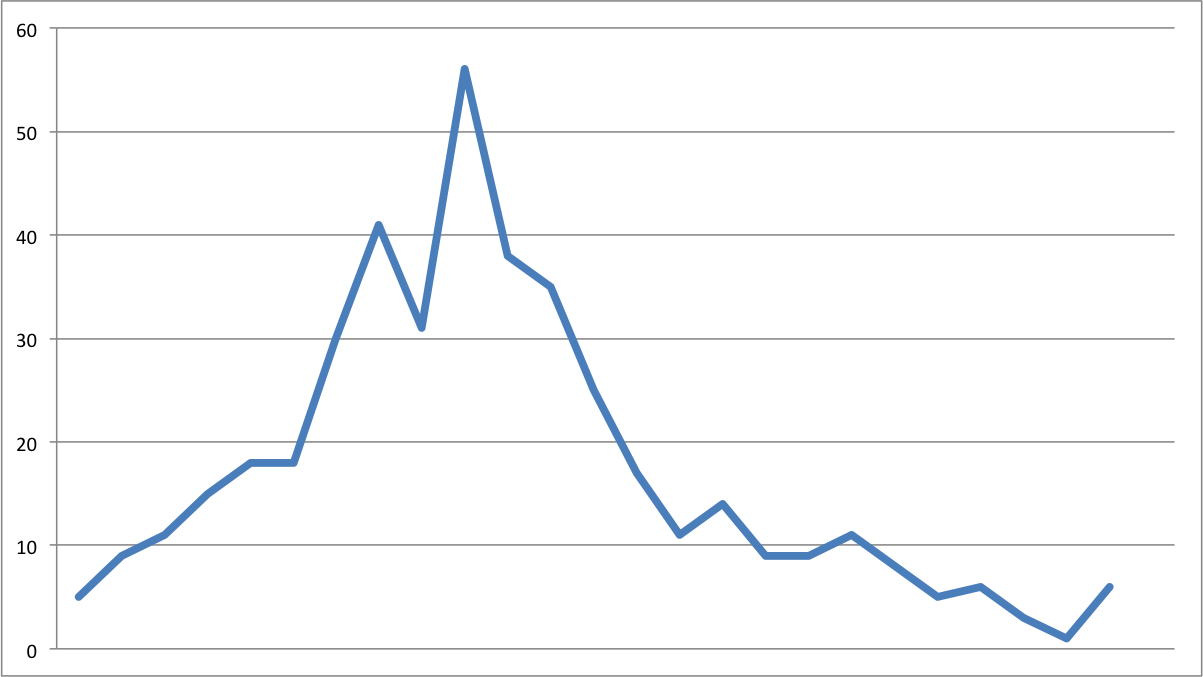
\includegraphics[width=4in]{../images/train_interarrivals/eastbound_blue_interarrivals.png}
\caption{\small \sl Eastbound Blue Line Interarrivals at Rosslyn. Ranges from 2.71 minutes to 16.78 with mean 10.91 minutes \label{fig:eastboundblueinterarrivals}}
\end{center}
\end{figure}

\begin{figure}
\begin{center}
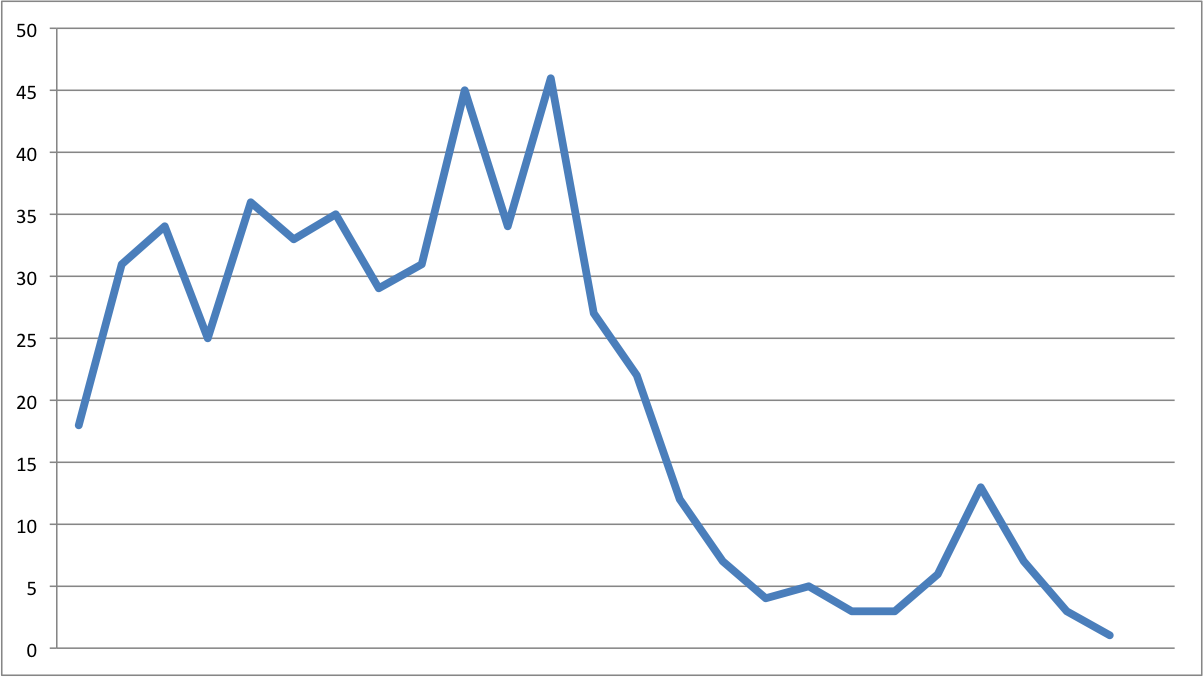
\includegraphics[width=4in]{../images/train_interarrivals/westbound_silver_interarrivals.png}
\caption{\small \sl Westbound Silver Line Interarrivals at Stadium-Armory. Ranges from 2 minutes to 24 with mean 9.25 minutes \label{fig:westboundsilverinterarrivals}}
\end{center}
\end{figure}

Time between stations results were fairly predictable, and most stations averaged around a 2 minute travel time between
stations. However, between Foggy Bottom and Rosslyn the times instead average around a minute higher. This is simply
due to the distance between the stations, which is considerably greater between those stations.

\section{Caveats and Limitations}
With any sort of simulation of a real-world system, there are simplications and assumptions that are made, and this project is of course no
different. In some cases the reduction in detail does not harm accuracy but simply makes the model designer's and
programmer's life easier. However, sometimes this is not the case and the simplifications greatly reduce the accuracy
of the model. Thus, it is the modeler's job to judiciously choose which details to omit and leave in when building the
model.

One of the simplifications that we've made is that we've excluded all other stations in the metro system except those
between Rosslyn and Stadium Armory. Other lines, the Red, Green, and Yellow lines, do not share track with any train,
nor do they cross at any point. In this respect, they are isolated. Event though other lines may share stations, the
trains run at a different elevation and therefore do no share a track. So, in this case, the simplification hinders
accuracy in no way whatsoever. However, ignoring Blue, Orange, and Silver stations beyond Stadium-Armory and Rosslyn
could potentially
reduce model accuracy here because train events at those stations can very easily influence the stations within D.C.
We have chosen instead to model those exterior stations as a probability distribution which is based off of empirical
data, but we still run a risk that we may have not captured an important interaction.

That being said, choosing an empirical distribution like we have has the potential to be a wise or poor choice. If the
"true distribution" of train interarrivals and between station times abides by what we have observed, then our choice
of empirical distribution was smart, and we've saved ourselves some effort. However we don't know the true
distribution, and it could be that our observations do not match that distribution at all.

For individual trains, we'll also ignore some of the micro-effects of acceleration and deceleration and assume our
between station times measurements captures that. For visualization purposes, we can simply draw trains as moving at a
constant velocity through the system, although this is clearly not the case.

\section{Technology Used}
The simulation was built using CoffeeScript \cite{coffeescript}, Backbone \cite{backbone}, Underscore
\cite{underscore} and jQuery \cite{jQuery} to organize code some. Code was bundled via Browserify \cite{browserify},
and minified with UglifyJS \cite{uglify}. Gulp \cite{gulp} was used as a build tool and NPM \cite{npm} was used as a
package manager. Geo-mapping was provided by Leaflet \cite{leaflet}, which has an API for enhancing the map with
markers, text, shapes, etc.

In an effort to ensure that the code worked properly, the simulation was built with a testing suite. Mocha \cite{mocha}
was used as the testing framework, and Chai \cite{chai} was used for BDD-style assertions. Sinon \cite{sinon} was used
to mock function calls during tests.

\section{Current Build and Instructions}
The functioning simulation is currently hosted at \cite{aprilandchip}. On this page, you can see trains moving through
the metro system, with real-time statistics as trains reach the other side. Also, tracks can be disabled via the
checkboxes at the bottom, which will influence trains in real-time. The map itself is interactive, and provides a few
glimpses into the system. Clicking on a station gives you the name, and clicking on a connection tells you current stats
at that section of track.

Also within the project directory that has been uploaded with the submission are some of the data analysis tools I've
built for performing queries, and cleaning data. These can be found in the \texttt{queries} and \texttt{utils}
directory of the project. Among the scripts found include bash scripts for file templating (for building queries
dynamically), templated js scripts for querying a mongo database, along with a few Python scripts for performing data
cleanup (like boxcar filtering for smoothing, and simple binning for histograms).

\section{Results and Conclusions}
One of the goals for this project was to better understand the metro system as a whole. In particular, I wanted to
discover how accurate WMATA was at predicting trains, and also how robust their scheduling was to unpredicted track
unavailability. WMATA provides their own estimates of how often trains occur \cite{metroschedule}, along with between
station times from any station to another \cite{rosslyntime}. This gives us plenty of room for comparison.

Empirically measuring between station times is a very granular way to measure the accuracy of WMATA's predictions. For
instance, stations within DC are estimated between 1 and 2 minutes, resulting in a travel time from Rosslyn to
Stadium-Armory taking 21 minutes. Based on the between station data we collected, we estimate empirically this actaully
ends up being around 24 minutes and 8 seconds. This discrepancy can be explained by a few reasons, the first being that
WMATA is wrong. This is of course, a potential case, but I'm more sure that this really an indication of issues in the
dataset itself. Since rail predictions are only precise to the minute, stations that are only a minute apart have the
potential to cause aliasing when calculating between station times. This may be the reason some of the interior station
times are 2 minutes instead of 1. Moreover, because this was a global measurement over a period of time, I may have 
captured some delaying event that caused between station times to diminish to a great enough value for a long enough
time to ``pull'' the mean up.

Regardless of these discrepancies, the simulation appears to agree with the estimates. Trains moving westward average
around 22.15 minutes to reach Rosslyn from Stadium-Armory within the simulation. Eastward trains perform slightly
better, hovering closer to 21 minutes. Both distributions, without any track disturbances, are very tight with little
variance. The difference in  means is accounted for by the empirical measurement of between station times. The total
westward time from Rosslyn to  Stadium-Armory is roughly 30 seconds shorter than the eastward counterpart. This could
be a result of many factors, such as geography, or even interactions beyond Rosslyn and Stadium-Armory ``captured''
in our empirical distribution. The remaining time may be accounted for by the Rosslyn-Foggy Bottom connection, the
most western connection in the system. The between station time here is  consistently 3 minutes, rather than 2.
Because of this, arriving trains may be forced to wait more often. WMATA estimates the travel time being the same
regardless of direction, and I still cannot explain the discrepancy.

Unsurprisingly, WMATA plans its trains effectively to be robust to a fair amount track outages, while still providing
the timings estimated on their website. Even with three tracks disabled, the mean travel time of eastern and western
trains still hovers around 23 minutes and 30 seconds. However, worth noting is that the \emph{variabilty} increases
drastically. Even though the mean moves little, there still are some trains that end up taking over 40 minutes to
reach the other side given these conditions. In a way, this is simply ``bad luck'' on that particular train's part,
simply because it's timing fell so that it arrived right as another train had occupied the track (with potentially
other trains waiting already). However as more tracks become disabled, the bad luck slowly becomes more likely for any
train to experience. Eventually, the mean does increase to around 32 minutes, with a very wide distribution with many
trains exceeding 45 minute travel times.

In conclusion, we see that WMATA does indeed provide fairly accurate estimates of train travel times, along with the
interarrival times between stations. Furthermore, WMATA's train scheduling is fairly robust to track outages, without
drastically impacting the throughput of trains. There are some unanswered questions, however. Why does the direction
affect the travel time between stations? Why do the simulated travel times agree with WMATA's estimate, but the average
interarrivals measured from the API do not? Would increasing the scope of the model improve the accuracy and remove the
discrepancies altogether? These questions can perhaps be answered with deeper investigation and more data.

\bibliographystyle{plain}
\bibliography{main}

\end{document}
